\chapter{Pre and post processing work preparation}
\label{Chapter2}

\section{Introduction}

This chapter focuses on the proposed methodology for analysing the mechanical fracture tests. It comprehensively explains the equipment for conducting the tests and the necessary preparations. A dedicated section is devoted to elucidating the application of the DIC method and the appropriate utilisation of MatchID software. Moreover, it outlines crucial DIC setting parameters, including subset size, step size, correlation criteria, and shape functions, to ensure optimal accuracy in the DIC analysis while balancing out the spatial resolution and precision.
Furthermore, this chapter introduces two fracture analysis methods, each accompanied by a custom-developed Python code. A comparative assessment of these methods is presented, allowing for a judgment regarding their relative effectiveness and merits.

\section{Material and testing}

\subsection{MMCG fracture test}

The MMCG specimen was initially developed by \citet{MoutouPitti2008}. However, it should be noted that the specimens tested in this work have different dimensions compared to the original design. Upon meticulous measurements, it was discovered that the tested specimens in this study share the exact dimensions as those examined by \citep{Odounga2018phd}. The dimensions of the specimens to be tested are provided in Figure \ref{fig:fig23}.

\begin{figure}[htp]
	\centering
	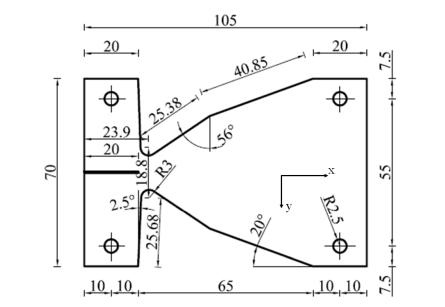
\includegraphics[width=.6\textwidth]{fig23}
	\caption{Dimensions of the tested MMCG specimen \citep{MoutouPitti2008, Odounga2018phd}.}
	\label{fig:fig23}
\end{figure}

\subsection{Wood characteristics}

For the tests conducted in this thesis, the chosen European species is the silver fir, which belongs to the category of coniferous trees. This softwood species is predominantly found in the northern hemisphere, similar to pines and other aged trees. Its name originates from the white colour of its wood, and its circumference typically ranges from 50 to 80 cm. According to CIRAD data, the silver fir exhibits a density of 0.45 to 0.60, a specific gravity factor (SFP) of approximately 30\%, and a compressive strength of 41 MPa. Notably, it experiences significant tangential shrinkage at 8.7\%, while the radial shrinkage measures 4\%. Silver fir wood is commonly utilised for framing, columns, and light structures due to its strength, although it requires treatment to prevent fungal and insect attacks. However, water pockets within the tree and its susceptibility to splitting pose concerns that may limit the use of specific connectors in construction.
Wooden specimens were carefully characterised before testing by measuring weight, density, and moisture content. Before the tests, the samples were weighed, denoted as $M_H$, to determine their mass during testing. The wood density can also be derived from the sample's volume and mass. AutoCAD was employed to create a digital representation of the sample, enabling us to determine its theoretical surface, which can then be multiplied by the thickness to calculate the volume. The density of each sample can be determined by applying the formula $\rho = M/V$.
After testing, the specimens were placed in an oven set at 100 degrees until their mass, labelled as $M_C$, stabilised. Two specimens were subjected to this process for 73 hours, and various measurements were taken until a constant mass was achieved. The moisture content of the specimens can be determined using Equation \ref{eq:HI}. Consequently, we possess the mass, density, and moisture content values necessary to compare our results with the literature review, as presented in Table \ref{tab:Tabmean}.

\begin{table}[h]
	\centering
	\begin{tabular}{lcl}\toprule
		Mass of the specimens, MH [g] && 29.83  \\
		Volume, V [cm$^3$] && 6916  \\
		Density, $\rho$ [kg/m$^3$] && 431.3  \\
		Moisture Content, HI [\%] && 10.3 \\\bottomrule
	\end{tabular}
	\caption{Characteristics of MMCG Silver Fir specimens.}
	\label{tab:Tabmean}
\end{table}

\subsection{Arcan solid model and grips}

An  Arcan fixture system is required to perform the  2MCG fracture tests. Indeed, this part allows the connection of the 2MCG wood specimen (Figure \ref{fig:fig23}) to the cross-head displacement of the test frame. Figure \ref{fig:fig24} shows the Arcan device we will use, inspired by the thesis of \citep{Odounga2018phd}.


\begin{figure}[htp]
	\centering
	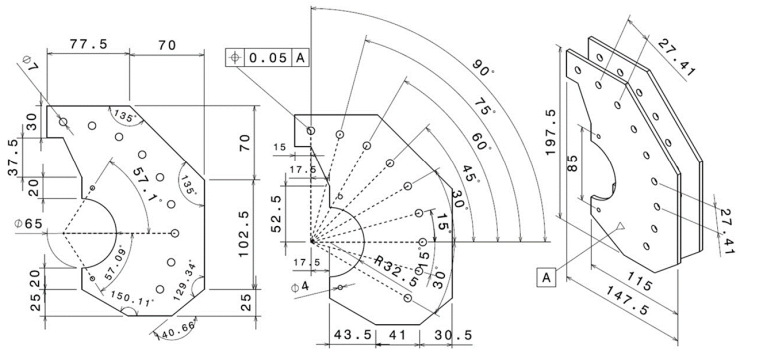
\includegraphics[width=15cm]{fig24}
	\caption{Size of the Arcan fastening system \citep{Odounga2018phd}.}
	\label{fig:fig24}
\end{figure}

The fixing holes for the wooden specimens have a diameter $\Phi= 4 mm$, and the loading holes have a diameter $\Phi = 7 mm$. These fixing holes were drilled in order to be able to load the specimen with different angular values of the angle in relation to the vertical direction in order to activate different failure modes depending on the load angle. To connect the Arcan system to the press, a piece had to be created, as shown in Figure \ref{fig:fig25}.


\begin{figure}[htp]
	\centering
	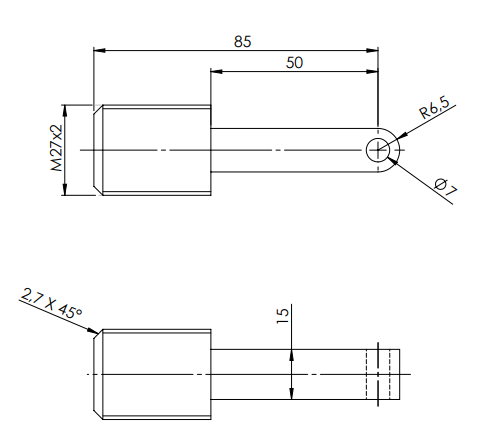
\includegraphics[width=6cm]{fig25}
	\caption{Bolt for connecting the press and the Arcan System.}
	\label{fig:fig25}
\end{figure}

This component incorporates a hole with dimensions identical to the Arcan specimen, facilitating seamless integration. Furthermore, the connector head has a diameter of 27 mm, and the thread has a pitch of 2 mm to ensure compatibility with the testing machine. The fixture was designed and assembled using SolidWorks software, and detailed technical drawings were produced for manufacturing (Figure \ref{fig:fig26}). However, before final production, a 3D printer was employed to create a prototype of the object, allowing for thorough verification and validation.

\begin{figure}[htp]
	\centering
	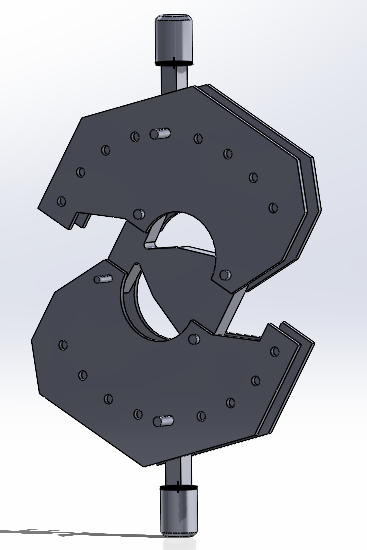
\includegraphics[width=7cm]{fig26}
	\caption{Assembled device in Solidworks.}
	\label{fig:fig26}
\end{figure}

Previous studies, including the work by \citep{Odounga2018phd}, have demonstrated a prominent issue associated with the MMCG specimen: the limited distance between the holes and the specimen extremities. This proximity leads to the formation of multiple cracks in the heel region between the hole and the sample's extremity, hindering practical observation and fracture analysis. To address this challenge, one proposed solution involves using washers that can be affixed through adhesive bonding or secured with robust screws and nuts. By applying compressive stress on each side of the sample, the stress applied to the holes is diminished, and the load is distributed across a broader area, thereby alleviating the issue.

\subsection{Universal testing machine}

The tests were conducted using a Landmark Servohydraulic Test Systems model 661.21B-03 from MTS, which served as the universal testing machine. This equipment can apply a maximum load of 100 kN (refer to Figure \ref{fig:fig27}). Displacement control was employed during the tests, with a cross-head displacement rate set to 0.1 mm/min. Data acquisition occurred at a frequency of 5 Hz. It is worth noting that in the study conducted by \citep{Mambili2018}, tests were performed at a frequency of 10 Hz, with a velocity of 0.3 mm/min and a pre-load of 100N. A pre-load was required to mount the specimen and fixture to the testing machine. However, the value of the pre-loading was considered in evaluating the energy release rate.

\begin{figure}[htp]
	\centering
	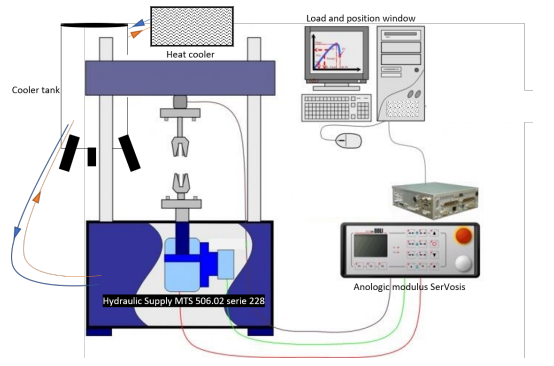
\includegraphics[width=10cm]{fig27}
	\caption{Hydraulic Press components allowing it use \citep{MALFAIT2021}.}
	\label{fig:fig27}
\end{figure}

\section{DIC method and setting parameters}

\subsection{Preparation of the DIC method}

Digital image correlation (DIC) enables the generation of displacement and strain maps, providing valuable kinematic information. The MatchID DIC 2D software was used in this study, and Python-based scripting was coded for post-processing purposes.
The focus of this study was the evaluation of crack opening displacement and crack length variation during the fracture tests with regard to the applied load. A monotonic optical system, employing a single camera, was employed. A speckle pattern was manually applied to all specimens using white-and-black spray paint to facilitate DIC analysis. The procedure involved initially applying a thin layer of white paint using a matte spray, followed by applying black paint to create a distinctive local pattern across the region of interest (ZOI) ahead of the crack tip. Notably, care was taken during lens and camera adjustments to optimise focusing and exposure time, ensuring an appropriate spread of light intensity to prevent pixel saturation in the sensor.

\subsection{MatchID}

In DIC processing, several steps are required:

\begin{itemize}
	\item Choose a reference image that corresponds to the first image of the test 
	\item Select multiple deformed images
	\item Define the zone of interest (ZOI) in which the crack propagates
	\item Define the  DIC setting parameters
	\item Start the DIC analysis
	\item Exploit the results
\end{itemize}

It is important to highlight the significant impact of both extrinsic and intrinsic setup parameters in digital image correlation (DIC), including subset size, subset step, strain gauge window, shape functions, and correlation criterion. These parameters play a crucial role in determining the calculated strain fields, resulting in variations in spatial resolution and resolution values that can differ by an order of magnitude or more \citep{DICguide2018}. The following paragraph aims to provide an explanation of some of these parameters.

\begin{itemize}
	\item The \textbf{correlation criterion} defines the matching criterion that will be adopted to determine the corresponding optimum point. In this work, ZNSSD criterion was selected. It is a least-square-based correlation criterion less sensitive to image contrast reduction and light intensity shifting between images.
	\item There are several \textbf{subset shape function} that the user can specify among rigid, affine and quadratic. Depending on the local deformation or strain gradients of the problem under analysis, the user can select affine or quadratic shape functions in the DIC method \citep{PereiraandXavier2018}.
	\item The \textbf{subset size} ($SS$) defines the spatial displacement resolution by specifying the correlation domain, that is, the number of pixels used to estimate a displacement vector. As a rule of thong, the region must contain at least three speckle light intensity variations. As an indication, larger subsets improve resolution but decrease spatial resolution. This means that in a conventional mechanical tensile test with a uniform, uniaxial stress state in the central region of the specimen, large subsets can be selected to improve the accuracy of the measurements. Nevertheless, the opposite is verified in fracture mechanics since the event of interest is relatively localised at the crack tip location.
	\item The \textbf{step size} ($ST$) refers to the amount of overlap between subset domains and determines the data points utilized in reconstructing the strain field. It plays a critical role in defining the spatial resolution of strains, meaning it controls the density of points at which DIC data is computed along a given length. Generally, setting the step size between one-third and one-half of the subset size is recommended, allowing for partial overlap between neighbouring subsets. However, it is important to note that this value can vary significantly depending on the specific application. In certain cases, a small step size may be necessary to accurately capture the peak position of a quantity of interest (QOI) within the ZOI, mainly if the QOI exhibits rapid variations without interpolation. Conversely, a larger step size can be used when the QOI changes gradually across the ZOI. The choice of step size should be carefully considered based on the specific requirements and characteristics of the investigated strain field.
	\item The \textbf{strain window} ($SW$) refers to the number of data points used to reconstruct the optimal polynomial function, using the least-square method, for calculating the analytical derivatives of strain components from the displacements. The selection of parameters such as subset size, step size, and strain window determines the spatial resolution of strain and the virtual strain gauge (VSG) characteristics.
	\item The \textbf{VSG} (virtual strain gauge) serves as a measure of spatial strain resolution and is calculated using the formula: $VSG=[(SW-1)\times ST] + SS$. The dimensions of the $VSG$ have an
    impact on the smoothness of the obtained results. Larger VSG dimensions yield smoothed results: however, the signal may be significantly underestimated in regions with heterogeneous deformation and
    significant gradients. On the other hand, a smaller $VSG$ provides data with higher noise levels but can better capture gradients. It is important to note that the pixel dimensions of the strain window are influenced by the chosen subset size and step size in the correlation algorithm. For instance, if a step size of 21 pixels is used, the availability of experimental displacement values is limited to every 21 pixels in both the horizontal and vertical directions. Consequently, an $N \times N$ strain window corresponds to a smoothing area with an actual width and height of
	[$(N-1) \times $ step size]+1 pixels. Furthermore, the displacement data points at the edges of the strain window are influenced by pixels extending beyond the dimensions. Therefore, determining strain values incorporates the subset size and should be considered accordingly.
\end{itemize}

In order to determine the most appropriate DIC settings, the Performance Analysis module within MatchID was employed. This tool allows for the definition of a range of options to be utilized in a design of experiments study. Parameters such as subset size, step size, and strain window can be varied systematically to enable a comprehensive comparison of the reconstruction of displacement and strain fields.

Subsequently, data from each analysis were extracted in a matrix format for each acquisition step. These data were then subjected to further analysis using Python scripting, with the aim of evaluating fracture parameters within the scope of this study.


\section{Python}

Python is a widely used computer programming language renowned for its versatility and extensive range of applications. It is frequently employed in developing websites, software systems, task automation, and data analysis. Unlike some specialized programming languages, Python offers a broad scope, allowing for the creation of diverse programs to tackle various problems. Furthermore, Python's user-friendly syntax and approachable learning curve have contributed to its widespread adoption, making it one of the most popular programming languages today.

An additional data processing step is required to determine the precise position of the crack tip and calculate the corresponding crack opening displacements. This information will enable the subsequent plotting of force as a function of crack opening or crack length and the evaluation of the energy release rate ($G$) as a function of crack length ($a$). Two distinct methods for accomplishing this task will be described in the following sections.

\subsection{Method 1: Crack propagation based on full-field displacement fields provided by DIC}

\textbf{Database}

A Python database file is created to obtain information for each specimen, such as the initial crack tip, the thickness of the specimen and the chosen subset for $a_0$.

\textbf{Reading data}

The first lines of the main program consist of reading and synchronising with image acquisition, the force and the displacements of the testing machine. Moreover, DIC data in the form of a subset $X$ and $Y$ coordinates together with $U_X$ and $U_Y$ components of the displacements for each stage are also read to workspace variables.

\textbf{Crack tip opening displacement}

The Crack Tip Opening Displacement (CTOD) will be calculated by analysing subsets positioned just above and below the subset that initially defines the crack tip position ($a_0$) in the pre-crack propagation images (see Figure~\ref{fig:fig29bis}). The $a_0$ subset corresponds to a specific entry in row $m$ and column $n$ in matrix representation. Observing the subsets from top to bottom makes it possible to track the displacement of the crack tip and measure it accurately. The objective is to identify the most suitable pair of subsets sufficiently close to the crack for meaningful measurements without being too close or too far. Proximity to the crack ensures relevant information, while excessive proximity or distance may compromise the accuracy of measurements. Through the analysis of these displacements, the crack opening values at each step can be obtained.
\begin{figure}[htp]
	\centering
	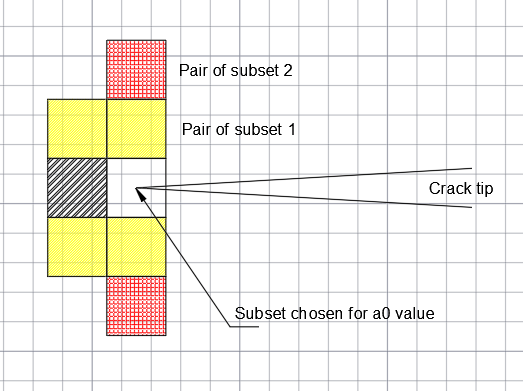
\includegraphics[width=8cm]{fig29bis}
	\caption{Pair of subsets around the chosen subset $a_0$.}
	\label{fig:fig29bis}
\end{figure}

\textbf{Mapping function and mapping mask}

The method used is based on the variation of the relative position between adjacent subsets, which gives an estimate of the damage occurrence \citep{Xavieretal2014}. To begin with, a matching function A(x,y) \ref{eq:eq21} is determined based on the norm of the relative position vectors as follows:

\begin{equation}
	A(x,y)=max(\lVert u_i-u_k\rVert;\lVert u_j-u_l\rVert)
	\label{eq:eq21}
\end{equation}

where $u_{i,j,k,l}$ represent the displacement vector of four adjacent subsets. A mapping mask \ref{eq:eq22} is then defined, assuming threshold segmentation according to the following inequalities.

\begin{equation}
	M(x,y)=
	\begin{cases}
		1, & \text{if } A(x, y) \geq \alpha \overline{A} \\
		0, & \text{if } A(x, y) < \alpha \overline{A} \\
		-1, & \text{if } A(x, y) = \textrm{NaN}
	\end{cases}
	\label{eq:eq22}
\end{equation}

The matrix $M$ serves as the basis for estimating the current horizontal location or crack length at a given stage. Zero values in the matrix indicate areas without a crack, while subsets within the crack or regions with missing information are assigned values of 1 and -1, respectively. Subsets surrounding the crack, which are of particular interest for the study, are assigned a value of 1. Constructing a sub-matrix consisting of -1, 0, and 1, one can visualise the damage evaluation as a map, providing an overview of the crack's development. Tracking the farthest subset with a value of 1 allows the determination of the last subset where the crack tip is located. To facilitate this, the parameter $\alpha$ acts as a cutoff tool, enabling the localisation of the crack position in the matrix coordinate space.

\textbf{$\alpha$ parameter}

The selection of the $\alpha$ parameter is not straightforward in the initial approach. To approximate its value, we first seek a correlation factor using the least squares regression method. During the test, the load-displacement curve consists of three main regions: a linear region representing a stationary zone, a second region corresponding to fracture propagation, and a third region indicating specimen rupture. By determining the correlation factor, we can identify the stage between the stationary zone and the Fracture Process Zone (FPZ). A second verification criterion based on displacement field processing is then applied to confirm the correct stage of the FPZ. By following these two steps, we can determine the stage at which the FPZ begins and the possible range of values for $\alpha$. Subsequently, we can plot the stages of crack propagation for different $\alpha$ values and assess the value of $\alpha$ that yields the largest $a(t)$ (crack length). Typically, the smallest $\alpha$ is chosen, unless a curve with simpler geometry is desired and the length of $a(t)$ remains relatively unchanged. A portion of the code enables graphical verification of the crack length by directly selecting $a_0$ and $a_f$ in Python. This allows the elimination of certain $\alpha$ values that do not yield the correct crack length..

\textbf{Crack length}

Another section of the code focuses on obtaining $a(t)$ as a function of $\alpha$. This is achieved by examining the ZOI and the subsets within it. By analysing the displacement field derived from each subset, the code calculates the distance between the centre of a subset and its displacement from one image to another. To simplify the code, this calculation is performed only on the four corner subsets. By measuring the distance between opposite corners, we obtain the maximum displacement in the $x$-direction and the displacement in the $y$-direction, which are then incorporated into a final matrix. Subsequently, the value of $a(t)$ is determined. It is equal to the initial crack length, $a_0$, specified by the user in the database, plus $\Delta a$, which represents the crack length variation over time in response to the applied force.


\subsection{Method 2: Crack propagation based on crack opening displacement provided by DIC}

Method 2 uses the crack opening along the entire length of the wooden specimen to determine the length of the crack (\citep{FilhoJ2022}). 

\textbf{Crack opening displacement (COD) or Virtual displacement}

From the reference and current positions of the DIC calculation points, the Euclidean distance between each pair of points can be measured and the COD can be determined as \ref{eq:eq23}:

\begin{equation}
	VD(k,i_n)=\sqrt{(x_{11bk}-x_{11tk})^2 + (x_{22bk}-x_{22tk})^2}_{i_n} - VD(k,i_0)
	\label{eq:eq23}
\end{equation}

where the indices t and b refer to the DIC data points located at the top and bottom of the crack path, k is the index of the DIC point, $i_n$ is the image captured at time n, VD(k, i0) is the initial Euclidean distance between the computational points of the top and bottom reference DIC subset obtained from image i0, and $x_{11}$ and $x_{22}$ are their coordinates in the image plane. VD can be defined as a displacement gauge along the crack path \ref{fig:fig30}.

\begin{figure}[htp]
	\centering
	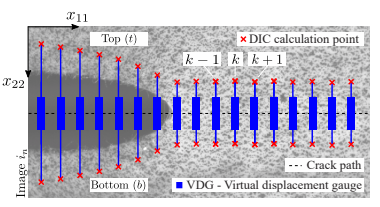
\includegraphics[width=10cm]{fig30}
	\caption{DIC-based virtual displacement gauge (VDG) \citep{FilhoJ2022}.}
	\label{fig:fig30}
\end{figure}

\textbf{$\alpha$ and $\beta$ parameters}

The first step towards detecting the crack tip is to take the average value of VD for each stage, \ref{eq:eq24}:

\begin{equation}
	\overline{VD}(i_n)=\frac{1}{k} \sum_{k=1}^{k}VD(k,i_n)
	\label{eq:eq24}
\end{equation}

The threshold value must be adjusted using the two parameters $\alpha$ and $\beta$ which are obtained by solving the equation \ref{eq:eq25}:

\begin{equation}
	\begin{cases}
		VD_{th}(i_1)=\overline{VD}(i_1)(\alpha i_1 +\beta)\\
		VD_{th}(i_f)=\overline{VD}(i_f)(\alpha i_f +\beta)\\ 
	\end{cases}
\label{eq:eq25}
\end{equation}

In order to obtain $VD_{th}(i_1)$ and $VD_{th}(i_f)$, it was first necessary to read graphically the position of the crack tip of the first and last image and then to find the intersection between the position of the crack tip and the crack opening VD for those two stages.

Therefore, the adjusted threshold line-cut $VD_{th}(i_n)$ is given by \ref{eq:eq26}:

\begin{equation}
	VD_{th}(i_n)=\overline{VD}(i_n)(\alpha i_n +\beta)
	\label{eq:eq26}
\end{equation}

The intersection between each $VD_{th}(i_n)$ and the corresponding $VD(k, i_n)$ curve at time n represents the $x_{11}$ position of the crack tip, denoted by ($p_n$).
It is therefore possible to calculate the growth of the crack at instant n \ref{eq:eq27}:

\begin{equation}
	da_n=p_n-p_0
	\label{eq:eq27}
\end{equation}

\subsection{Difficulties in applying method 2}

This method was originally used for a fibrous soft material. The first step was to translate the Matlab code given by \citep{FilhoJ2022} into a python code to be able to use both methods simultaneously and compare them.
After translating the code, we realised that this method did not work properly for the wood material and the DIC data we had with Stanislas' tests.
From the data of method 1, we already know the position of a0 and all the displacements over time that have occurred on the entire wooden specimen. However, for method 2, we only need 2 horizontal lines placed above and below the fracture. It is therefore sufficient to take only one part of the data from the specimen. Moreover, it was chosen to take these two lines far enough away from the fracture in order not to have subsets without any data.
However, method 2 still didn't work properly and a slight modification to the code was required.

The Figure \ref{fig:fig31} corresponds to the plot of $\overline{VD}$ and $VD_{th}$ with Joao's data, the author of the method. We read graphically $a_1$ and $a_f$, which allowed us to know the $VD_{th}$ for index 1 and the last index which are the bounds on the y-axis for the $VD_{th}$ curve. We notice that the $VD_{th}$ curve has the same shape as the $\overline{VD}$ curve, is still increasing but has only been reduced at the ordinate level. This is what we want to achieve for the MMCG specimens.

For the MMCG test data, by applying $VD_{th1}$ and $VD_{thf}$ as in Joao's data, we notice that the $VD_{th}$ curve increases and then decreases, which is not normal since the COD should normally increase with time (figure \ref{fig:fig32}). This is due to the alpha and beta factors which increase $\overline{VD}$ for the first indices and then decrease $\overline{VD}$ for the last indices. According to the equation \ref{eq:eq26} alpha is multiplied by $i_n$ which will decrease the multiplier coefficient of $\overline{VD}$ over time if alpha is negative and beta positive. This is the reason why $VD_{th}$ is under $\overline{VD}$  for the latest indices.

\begin{figure}[htp]
	\begin{minipage}[c]{.46\linewidth}
		\centering
		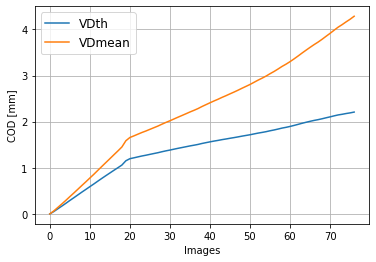
\includegraphics[width=7cm]{fig31}
		\caption{$\overline{VD}$ and $VD_{th}$ with Joao's data.}
		\label{fig:fig31}
	\end{minipage}
	\hfill%
	\begin{minipage}[c]{.46\linewidth}
		\centering
		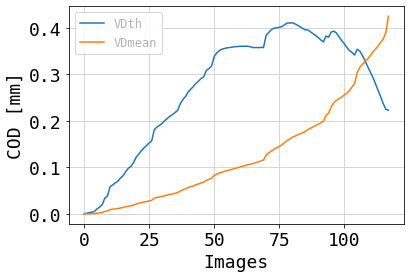
\includegraphics[width=7cm]{fig32}
		\caption{$\overline{VD}$ and $VD_{th}$ with stanislas' data.}
		\label{fig:fig32}
	\end{minipage}
\end{figure}


Method 1 was then used to find out from which image the fracture process starts. Method 2 directly increased the length of the crack for the first images, which is not normally the case for wood.  Indeed, it is considered that for all the images before the FPZ there is a(t)=a0. We therefore read $a_1$ and $a_f$ with $a_1$ the index of the beginning of the fracture process and $a_f$ the last image before the material breaks. The graph \ref{fig:fig33} is then obtained.


\begin{figure}[htp]
	\centering
	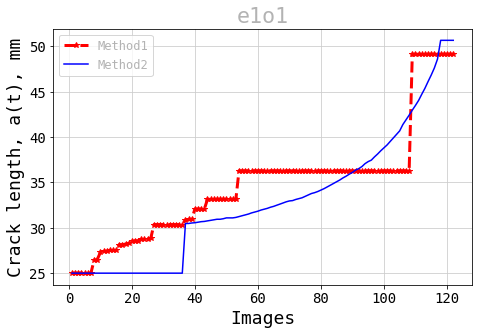
\includegraphics[width=7cm]{fig33}
	\caption{Crack length with FPZ taken into account.}
	\label{fig:fig33}
\end{figure}

The fracture for method 2 starts much later than method 1 and are different over the time. Furthermore, the crack length does not end at the same place, because for method 2 the fracture at the last index is read graphically which is less accurate.
Because the $\overline{VD}$ is too small compared to the graphically obtained $VD_{th1}$, an interpolation is made to increase the $\overline{VD}$. The graph \ref{fig:fig34} is obtained:

\begin{figure}[htp]
	\centering
	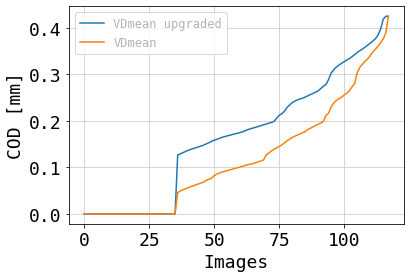
\includegraphics[width=7cm]{fig34}
	\caption{Interpolation of $\overline{VD}$.}
	\label{fig:fig34}
\end{figure}

Thanks to this interpolation, we apply alpha and beta (figure \ref{fig:fig35}) and obtain $VD_{th}$. Finally, we obtain the crack length graph \ref{fig:fig36}:

\begin{figure}[h]
	\begin{minipage}[c]{.46\linewidth}
		\centering
		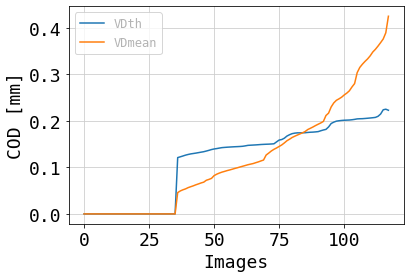
\includegraphics[width=7cm]{fig35}
		\caption{$VD_{th}$ with interpolation.}
		\label{fig:fig35}
	\end{minipage}
	\hfill%
	\begin{minipage}[c]{.46\linewidth}
		\centering
		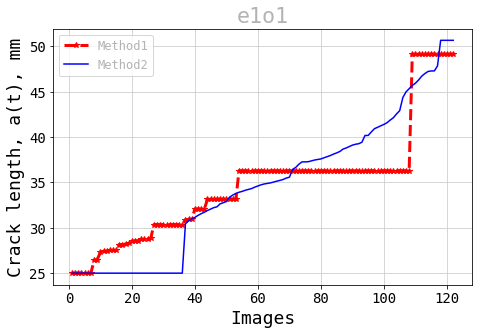
\includegraphics[width=7cm]{fig36}
		\caption{Final crack length e1o1.}
		\label{fig:fig36}
	\end{minipage}
\end{figure}

To conclude, the crack propagation does not start at the same stage between the two methods and the crack length is different over the time. Moreover we had to modify a lot Joao's initial method to apply it to wood material. It also adds uncertainties since we have to read graphically $a_1$ and $a_f$ to obtain the crack length thresholds at the beginning and at the end of the propagation. Reading the points $a_1$ and $a_f$ is really difficult to evaluate manually for this material because the fracture is not clearly visible on the images. In addition, the index for $a_1$ and $a_f$ is given by method 1 which adds further uncertainties. Method 2 gives a "smoother" curve than method 1, but this is not necessarily a good thing since the fracture of wood material usually works in fits and starts.
As observed in method 1, the fracture process typically involves multiple stages, which can be attributed to the gradual propagation of cracks. In some instances, the presence of bridges in the material can impede the linear advancement of the crack. However, once these bridges break, the crack can propagate further, resulting in the development of a new stage in the fracture process. This underscores the complex nature of crack propagation in wood. In the next chapter, the tests carried out in mode I will be presented and we will be able to check whether method 2 works correctly with wood. However, some doubts are raised, as the $\overline{VD}$ is not as linear as with a soft fibrous material, as shown in Figures \ref{fig:fig31} and \ref{fig:fig32}.

\subsection{Energy release rate}

After using one of the two previous methods, we can calculate the energy release rate in mode I and in mixed mode.

For mode I, the formula is the one explained in \ref{eq:eq125}.

For mixed mode, the formula becomes \ref{eq:eq28}:

\begin{equation}
	\begin{cases}
		G_I=\frac{{F_{cy}}^2}{2b}\ \frac{\partial C_I}{\partial a} \quad \text{with } C_I=\frac{v}{F_{cy}} \\
		G_{II}=\frac{{F_{cx}}^2}{2b}\ \frac{\partial C_{II}}{\partial a} \quad \text{with } C_{II}=\frac{u}{F_{cx}}\\ 
	\end{cases}
\label{eq:eq28}
\end{equation}

where u and v are the crack opening displacement according to x and y. The displacement measured by the machine is not used to calculate the energy release rate, as it is less accurate due to the clearances in the jaws.

In mixed mode the camera will have the same inclination as the specimen Figure \ref{fig:fig37bis}.

\begin{figure}[htp]
	\centering
	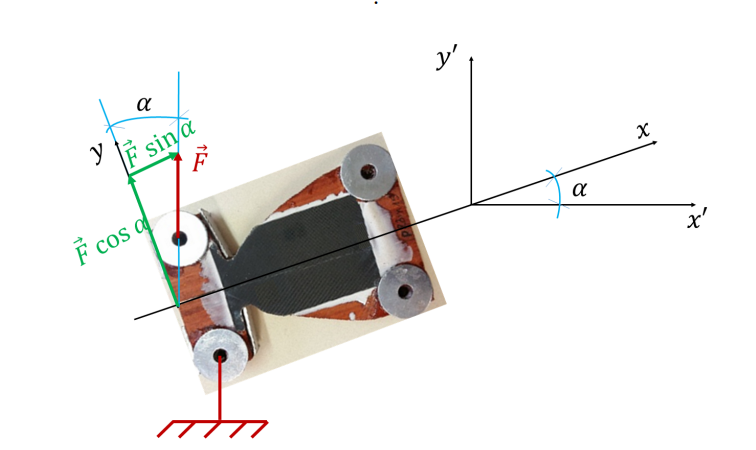
\includegraphics[width=9cm]{fig37bis}
	\caption{Force projection along the axes in mixed mode, \citep{Odounga2018phd}.}
	\label{fig:fig37bis}
\end{figure}

The crack opening values will therefore be projected directly along the x and y axes. The force is projected along the x and y axes, so we have \ref{eq:eq29}:


\begin{equation}
	\begin{cases}
		F_{cx}=F \sin(\alpha) \\
		F_{cy}=F \cos(\alpha) \\ 
	\end{cases}
	\label{eq:eq29}
\end{equation}


\section{Specimen preparation}

\subsection{Specimen names}

We have 20 specimens of silver fir of 12.5mm thickness.
We will therefore use 5 specimens per degree of inclination. This means 5 specimens in pure mode I (0°) and 15 specimens in mixed mode (15°, 30°, and 45°).
Naming the specimens allows to know which test was performed on which specimen. The first part of the name corresponds to the inclination of the specimen during the test using the Arcan system:
\newline
E0 : Test in pure mode I
\newline
E15 : Test with specimen tilt of 15°
\newline
E30 : Test with specimen tilt of 30°
\newline
E45 : Test with specimen tilt of 45°


E15, E30 and E45 are therefore the specimens tested in mixed mode.
Then the name as a second component is the number of the specimen dedicated to this test.
Finally, all samples are named as E0E1 which is the first sample used in pure mode.

\subsection{Notch and precrack}

Notches were created in each specimen. A precrack is made by a cutter into the notch. The interest is to initiate a straight crack, thanks to this first one. The notch width is around 1.5mm, done by a straight electrical saw. The cutter allow to go deeper and create a precrack with a shape that allows the propagation of the crack. The precrack must be done at the center of the sample heel. Indeed, even a little eccentricity could cause a deviation of the crack and prevent a good study of the propagation. The specimen was designed with an initial crack noted $a_i$ and the total crack length is equal to: $a=a_i+\Delta a$.

The initial crack lengths are obtained by averaging the notch on each side of the specimen plus the precrack also measured with the average of the two sides of the specimen.
The following initial crack length values are then obtained:

\begin{table}[h]
	\centering
	\begin{tabular}{c c }
		\multicolumn{1}{l}{} & \multicolumn{1}{l}{Initial Crack length} \\
		\multicolumn{1}{c}{\cellcolor[HTML]{F8CBAD}E0E1} & 25,3   mm \\
		\multicolumn{1}{c}{\cellcolor[HTML]{F8CBAD}E0E2} & 24.85 mm \\
		\multicolumn{1}{c}{\cellcolor[HTML]{F8CBAD}E0E3} & 25.65 mm \\
		\multicolumn{1}{c}{\cellcolor[HTML]{F8CBAD}E0E4} & 24,7 mm \\ 
		\cellcolor[HTML]{F8CBAD}E0E5 & 25,6 mm \\ 
		\cellcolor[HTML]{F8CBAD}E0E6 & 26,3 mm \\ 
		\multicolumn{1}{c}{\cellcolor[HTML]{C65911}E15E1} & 25,85 mm \\ 
		\multicolumn{1}{c}{\cellcolor[HTML]{C65911}E15E2} & 25,6 mm \\ 
		\multicolumn{1}{c}{\cellcolor[HTML]{C65911}E15E3} & 25,55 mm \\ 
		\multicolumn{1}{c}{\cellcolor[HTML]{C65911}E15E4} & 25.3 mm \\
		\multicolumn{1}{c}{\cellcolor[HTML]{C65911}E15E5} & 24,85 mm \\ 
		\multicolumn{1}{c}{\cellcolor[HTML]{BF8F00}E30E1} & 25,55 mm \\ 
		\multicolumn{1}{c}{\cellcolor[HTML]{BF8F00}E30E2} & 24,4 mm \\ 
		\multicolumn{1}{c}{\cellcolor[HTML]{BF8F00}E30E3} & 24,2 mm \\ 
		\multicolumn{1}{c}{\cellcolor[HTML]{BF8F00}E30E4} & 25,3 mm \\ 
		\multicolumn{1}{c}{\cellcolor[HTML]{BF8F00}E30E5} & 24.4 mm \\ 
		\multicolumn{1}{c}{\cellcolor[HTML]{BF8F00}E30E6} & 24.35 mm \\ 
		\multicolumn{1}{c}{\cellcolor[HTML]{BF8F00}E30E7} & 25.6 mm \\
		\multicolumn{1}{c}{\cellcolor[HTML]{FFA500}E45E1} & 25,8 mm \\ 
		\multicolumn{1}{c}{\cellcolor[HTML]{00FF00}broken} & 25.95 mm \\  
	\end{tabular}
	\caption{Precrack dimensions.}
	\label{tab:Tab11}
\end{table}

We can see that only one test was carried out at 45 degrees. Some tests were not successful. The tests for angles 0°, 15° and 30° were therefore preferred.

\section{Conclusion}

This chapter has given us a better understanding of all the tools used to carry out the tests. It also explains some parameters that are essential to the success of the DIC method. Finally, it presents two methods for evaluating crack length; one using full-field displacement and the other using COD.
According to the results from the two methods, method 1 appears to be more accurate than method 2. In the next chapter, we will be able to better evaluate the efficiency of the two methods.


